\documentclass[xetex,aspectratio=43]{beamer}

\usepackage{res/lections}

\preamble

\title[Устройство и принципы проектирования ЦП, конвейеризация]{Общее устройство центрального процессора, принципы его проектирования, конвейеризация}

\begin{document}

    \titleslide

    \tocslide

\section{Блоки процессора}

\begin{frame}{Арифметико-логическое устройство}
    \defn{Арифметико-логическое устройство}{блок процессора, выполняющий арифметические и логические операции}
    \begin{itemize}
        \item В простейшем случае --- просто логическая схема
        \item Может использоваться для прикладных (например, вычисления, заданные программистом) и служебных (например, адресная арифметика)
        \item Имеет несколько входов для операндов и выход, на который \emph{мультиплексируются} выходы сумматора, мультипликатора и т.д.
    \end{itemize}
\end{frame}

\begin{frame}{Регистровый файл}
    \defn{Регистровый файл}{блок процессора, включающий набор регистров; внутренняя память процессора}
    \begin{outline}[itemize]
        \tightlist
        \1 Арифметические регистры
            \2 Аккумулятор
            \2 Ещё несколько [десятков] регистров
        \1 Регистры состояний
            \2 Регистр флагов
        \1 Адресные регистры
            \2 Указатель вершины стека
            \2 Указатель на текущую инструкцию
            \2 Указатель на данные [часто несколько]
            \2 Вспомогательные (например, сегментные)
        \1 Служебные регистры
            \2 Хранение промежуточных значений, реализация протоколов (например, с ОЗУ) и т.д.
    \end{outline}
\end{frame}

\begin{frame}{Блок выборки инструкций (устройство чтения программы)}
    \defn{Блок выборки инструкций}{блок процессора, выполняющий чтение очередных инструкций из памяти}
    \begin{outline}[itemize]
        \1 Читает из ОЗУ машинный код
            \2 Выполняет первичную интерпретацию машинного кода
    \end{outline}
    Для CISC-процессоров со сложным машинным кодом это не так-то просто!

    \pause
    \alert{О том, что такое RISC и CISC, ещё немного позже.}
\end{frame}

\begin{frame}{Управляющее устройство}
    \defn{Управляющее устройство}{блок процессора, выдающий для исполнения машинных команд управляющие сигналы другим блокам}
    \begin{outline}[itemize]
        \1 В зависимости от команды, выдаёт управляющие сигналы другим блокам процессора
            \2 Сигналы преимущественно управляют мультиплексорами, т.е. задают \emph{маршруты передачи данных между блоками процессора}
        \1 Если команда выполняется за много тактов (а обычно так и есть), выдаёт не один сигнал, а \emph{последовательность сигналов} разным блокам
    \end{outline}
\end{frame}

\section{Одно-, многотактный процессоры}

\begin{frame}{Однотактная схема}
    \begin{figure}
        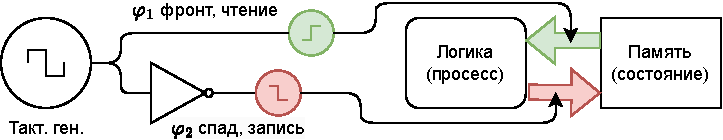
\includegraphics[width=\textwidth, page=1]{img/11.CPUS.drawio-crop.pdf}
    \end{figure}
    Вспоминаем:
    \begin{outline}[enumerate]
        \1 Синхронные и асинхронные вычисления, тактовый генератор, тактовые импульсы и тактовую сеть
        \1 Синхронизацию по фронту и спаду тактового импульса
        \1 Связку «master-slave»
        \1 Многофазные тактовые сигналы у старых процессоров
    \end{outline}
\end{frame}

\begin{frame}{Однотактный процессор}
    \begin{figure}
        \includegraphics[width=0.75\textwidth, page=2]{img/11.CPUS.drawio-crop.pdf}
    \end{figure}

    \begin{outline}[itemize]
        \1 В принципе, он даже может работать
            \2 Можно «нарисовать», например, несложный контроллер с такой архитектурой
        \1 Только гарвардский, т.к. нельзя одновременно обращаться и в одну память за кодом и данными
    \end{outline}
\end{frame}

\begin{frame}{Многотактный процессор (упрощённый пример для 3 тактов)}
    \begin{figure}
        \includegraphics[width=0.95\textwidth, page=3]{img/11.CPUS.drawio-crop.pdf}
    \end{figure}
\end{frame}

\begin{frame}{Как оно работает, и хорошо ли?}
    \begin{block}{Как?}
        \begin{outline}[itemize]
        \1 Используются три фазы --- $\varphi_0, \varphi_1, \varphi_2$
            \2 Эти фазы может генерировать процессор внутри себя по сигналам обычного тактового генератора
        \1 Простая (и не очень) логика реализуется на основе \emph{конечных автоматов} (удобный абстрактный вычислитель, помогающий решать конкретные задачи =) )
        \1 Сложная логика реализуется при помощи микрокода --- в -1 приближении --- последовательности (работает много тактов) управляющих сигналов для мультиплексоров на входах блоков процессора
    \end{outline}
    \end{block}

    \pause
    \begin{block}{Хорошо ли?}
    \begin{outline}[itemize]
        \1 Разные фазы выполняются разными блоками по очереди
            \2 $\frac{2}{3}$ времени блоки процессора простаивают!
    \end{outline}
    \end{block}
\end{frame}

\section{Конвейеризация}

\subsection{Конвейеры в реальной жизни}

\begin{frame}{Конвейеризация «в жизни»}
\begin{block}{Предпосылки}
    Эли Уитни, 1798 (оружейное производство) — одновременное изготовление стандартизованных узлов мушкета разными рабочими, затем быстрая сборка готовых изделий
\end{block}

\begin{block}{Реальные конвейеры}
    \begin{outline}[itemize]
        \1 Генри Форд, 1913 и т.д. — сборка электрогенераторов, затем моторов и целых автомобилей
            \2 Разные этапы производства выполняются разными рабочими
            \2 Рабочие работают одновременно, каждый на своём этапе
        \1 Конвейер в системе образования
            \2 Школа: 1–11 классы — выпуск каждый год, но школьник учится 11 лет
            \2 Высшее образование: \emph{старая} поговорка: Матмех — не школа, за \emph{10 лет} не окончишь =)
        \1 Конвейер в менеджменте
            \2 Конвейерное исполнение заказов
    \end{outline}
\end{block}
\end{frame}

\begin{frame}{Недостатки конвейера}
    \begin{outline}[itemize]
        \1 Низкая гибкость — организованный и запущенный конвейер тяжело приспособить к изменяющейся ситуации
        \1 Снижение качества результата в угоду массовости
            \2 Пример: товар есть на складе в моём городе, но почему-то едет с другого конца страны
    \end{outline}
    \pause
    Выход: в менеджменте это преодолевается переходом от конвейера к организации бизнес-процессов — сложнее, но адаптивнее
\end{frame}

\subsection{Вычислительные конвейеры}

\begin{frame}{Что такое конвейер?..}
    \defn{Вычислительный конвейер (водопровод, pipeline)}{механизм распараллеливания выполнения машинных команд, позволяющий оптимально задействовать блоки процессора путём разбиения команд на стадии и распределения стадий по блокам}

    ~

    Конвейеры появились в 1950-х годах, термин «конвейер» (pipeline) ввёл конструктор советских ЭВМ С.А. Лебедев.

    ~

    Пусть все команды выполняются за $N$ тактов. Тогда, что даёт конвейеризация?

    \begin{outline}[itemize]
        \1 Скорость выполнения отдельных команд:
            \2 Каждая команда выполняется за $N$ тактов как с конвейером, так и без
            \2 В отношении одной команды на разных тактах задействованы разные блоки
        \1 Скорость выполнения программы:
            \2 На каждом такте завершается очередная команда
            \2 Конвейеризация ускоряет работу программы в $N$ раз, все блоки задействованы всё время
            \pause
            \2 Косвенная выгода: «сосредоточение» отдельных стадий в компактных блоках позволяет увеличить тактовую частоту
    \end{outline}

\end{frame}


\begin{frame}{Пример: Classic RISC Pipeline}
    \begin{figure}
        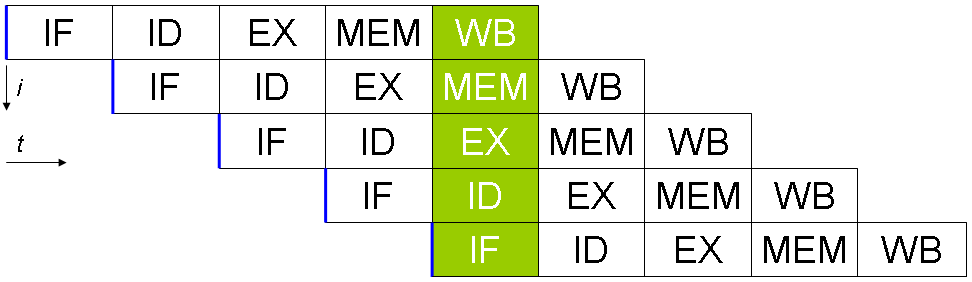
\includegraphics[width=0.7\textwidth]{img/11.classic-RISC-pipeline.png}
        \caption{Classic RISC Pipeline, Wikipedia}
    \end{figure}
    Применялся к популярным RISC-процессорам 1980-х: первым MIPS, Sun SPARC, Motorla 88000.
    Стадии:
    \begin{enumerate}
        \tightlist
        \item IF (instruction fetch) — получение инструкции
        \item ID (instruction decode) — декодирование инструкции
        \item EX (execute) — выполнение инструкции, если нужно — первый такт доступа к данным в ОЗУ
        \item MEM memory access) — второй такт доступа к данным в ОЗУ или бездействие
        \item WB (register write back) — запись в регистр
    \end{enumerate}
\end{frame}

\begin{frame}{Проблемы конвейеризации}
    \begin{outline}[enumerate]
        \renewcommand{\outlineii}{itemize}
        \1 Конфликты по данным между зависимыми машинными командами, например:
            \2 самая частая ситуация — следующей команде нужен результат предыдущей, но предыдущая ещё его не получила
            \2 следующая команда записывает данные до того, как их читает предыдущая
            \2 следующая команда записывает свои результаты раньше предыдущей из-за чего предыдущая потом может их перезаписать

        \1 Конфликты по ресурсам — когда двум командам одновременно нужен эксклюзивный доступ к чему-либо (регистр, шина\ldots)

        \1 Конфликты по управлению: следующая команда является условным переходом, но условие для него ещё не вычислено предыдущей командой
            \2 и даже не ясно, из какой ветви дальше выбирать команды
            \pause\\
            \alert{Спойлер: некоторые RISC процессоры, например ранние MIPS, исполняли до двух команд даже после \emph{безусловного} перехода: конвейер успевал из «засосать» из памяти, не успевая ещё разобрать, что в них}
    \end{outline}
\end{frame}

\begin{frame}{Решение проблем конвейеризации}
    \begin{itemize}
        \item Pipeline Stall — торможение команд на конвейере; в предельном случае может свести преимущества конвейеризации на нет
        \item Предсказание условных переходов — сбор статистики о переходах или подсказки от компилятора
    \end{itemize}
\end{frame}

\section{CISC- и RISC процессоры}

\subsection{Основы}

\begin{frame}[fragile]{Пример программы и её трансляции (1: x86)}
    \begin{center}
        \begin{minipage}{0.4\linewidth}
            \begin{minted}{C}
                int factorial(int n)
                {
                    int r = 1;
                    while(n > 1)
                    r *= n--;
                    return r;
                }
            \end{minted}
        \end{minipage}
    \end{center}

\href{https://github.com/dluciv/Computer_Architecture-SPbU-CB.5080/tree/main/examples/cross-compiling}{Примеры компиляции и кросс-компиляции} для x86, ARMv9, MIPS64, RISC-V

\end{frame}

\begin{frame}{Что отличало данные примеры?}
    \defn{Система команд}{соглашение о средствах, предоставляемых машинным языком и о структуре машинного языка}
    \begin{figure}
    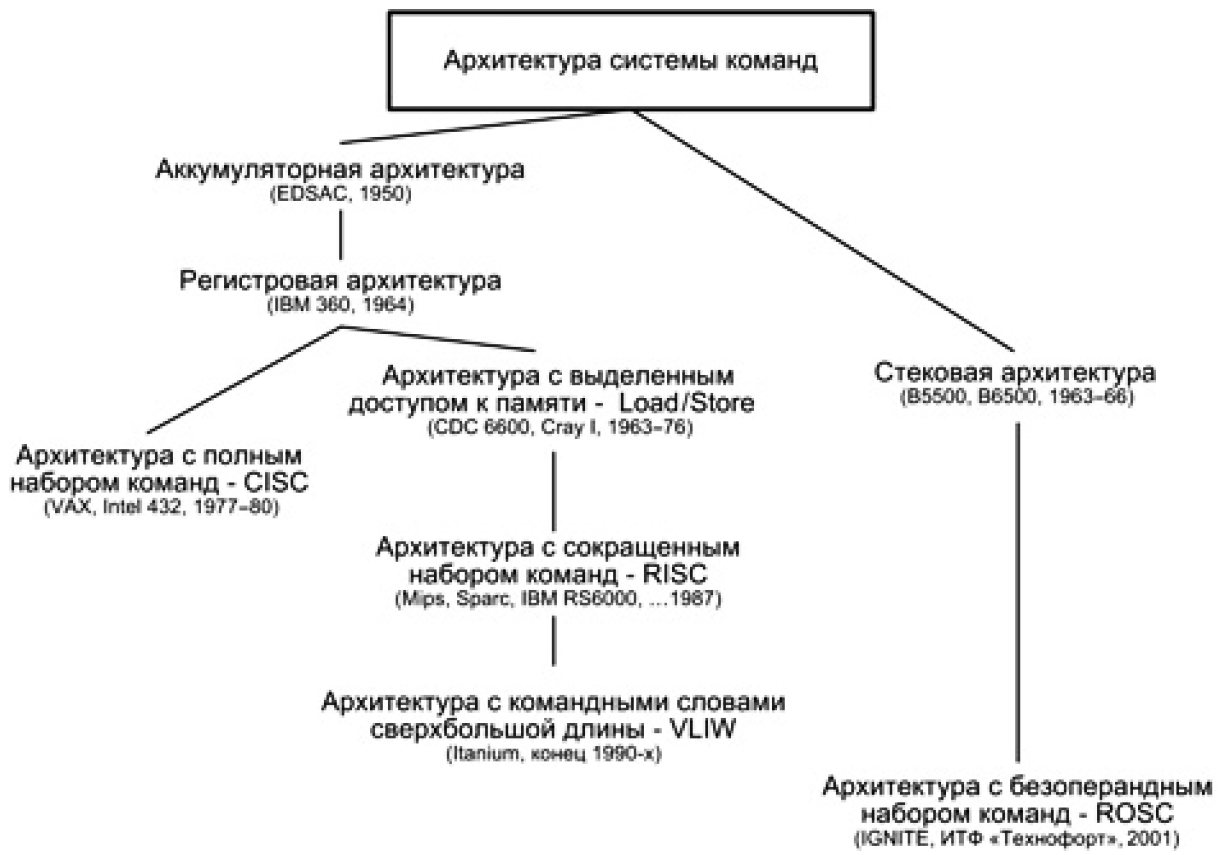
\includegraphics[width=0.7\textwidth]{img/11.instr_sets.png}
    \caption{Орлов С.А., Цилькер Б.Я. Организация ЭВМ и систем: Учебник для вузов. 2-е изд. — СПб.: Питер, 2011. — 688 с.}
    \end{figure}
\end{frame}

\begin{frame}{CISC}
    CISC — Complicated Instruction Set Computer

    \begin{outline}[itemize]
        \1 Много способов адресовать аргументы команд
            \2 Смешанная адресация — разные операнды из разных мест
            \2 Команды похожи на операторы языков высокого уровня
        \1 Ассемблер дружественный
        \1 Небольшое количество сильно умных команд
            \2 Реализованы при помощи микропрограмм
        \1 Машинный код экономный в смысле занимаемого места в памяти (многие «популярные» команды занимают 1 байт)
    \end{outline}

    Примеры:

    IBM/360..z-Architecture, Intel x86 и x86\_64, Intel 8080 и Zilog Z80
\end{frame}

\begin{frame}[fragile]{RISC}
    RISC — Reduced Instruction Set Computer

    \begin{outline}[itemize]
        \1 Отдельные команды для обмена данными с памятью
        \1 Команды простые
            \2 Команды выполняются за фиксированное время (фиксированное количество тактов)
            \2 Это упрощает конвейеризацию
        \1 Некоторые «долгие» команды выполняются асинхронно
        \1 Ассемблер недружественный
            \2 Помните про «глупый всеядный» конвейер?
        \1 Машинный код не экономный, все команды занимают одно машинное слово
            \2 В некоторых режимах половину (для RISC-V попробуйте \mintinline{sh}{-march=rv64g} vs \mintinline{sh}{-march=rv64gc})
    \end{outline}

    Примеры:

    Cray CDC 6600 (1960-е), и большинство новых семейств, начиная с 1980-х: MIPS, SPARC, ARM, RISC-V
\end{frame}

\begin{frame}{CISC vs RISC: недружественный ассемблер --- это очень страшно?}
    \pause
    \alert{Нет.}
    \begin{figure}
        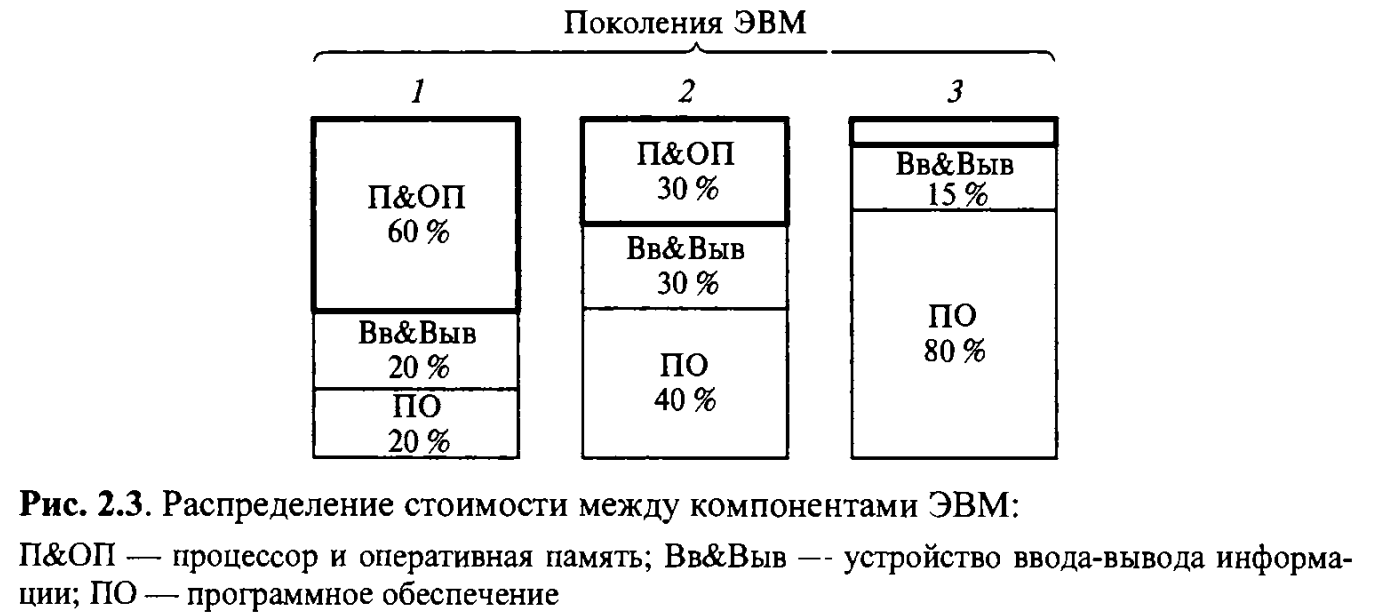
\includegraphics[width=0.8\textwidth]{img/11.generation_prices.png}
        \caption{Архитектура вычислительных систем.: Учеб. пособие. 2-e изд., перераб. и доп. M.: Изд-во МГТУ им. H.Э. Баумана, 2008. 520 c.}
    \end{figure}

    \begin{itemize}
        \item Cray CDC 6600 --- суперкомпьютер середины 1960-х, можно было программировать дорого, т.к. он и сам был очень дорогой
        \item Большинство --- 1980-е и позже, программируются уже на языках высокого уровня
    \end{itemize}
\end{frame}

\subsection{Особенности конвейеризации}

\begin{frame}{Конвейеризация в RISC}
    \begin{block}{Особенности и трудности}
        У RISC простой формат машинного кода, простой блок выборки инструкций, простой конвейер.
        Иногда есть несколько «долгих» команд, которые выполняются асинхронно
                \alert{Некоторые RISC-семейства не отслеживают конфликты и не обрабатывают их!}
    \end{block}

    \pause

    \begin{block}{Решения}
        \begin{itemize}
            \item Переупорядочивание команд — конфликтующие команды размещаются «на безопасном расстоянии» друг от друга
            \item Торможение при помощи вставки «пузырька» (инструкция nop, no operation)
        \end{itemize}
        \alert{Для некоторых RISC-семейств всё это делает компилятор или программист!}
    \end{block}
\end{frame}

\begin{frame}{Конвейеризация в CISC}
    Процессор полностью сам отвечает за корректное исполнение кода --- обнаруживает конфликты и обрабатывает их.

    ~

    Процессор с конвейером должен (кроме скорости) работать так же, как и без конвейера.
\end{frame}

\section{А мы же говорили, что конвейер не гибкий?..}

\subsection{Суперскалярность}

\begin{frame}{Суперскалярное исполнение: сущность}
    \begin{figure}
        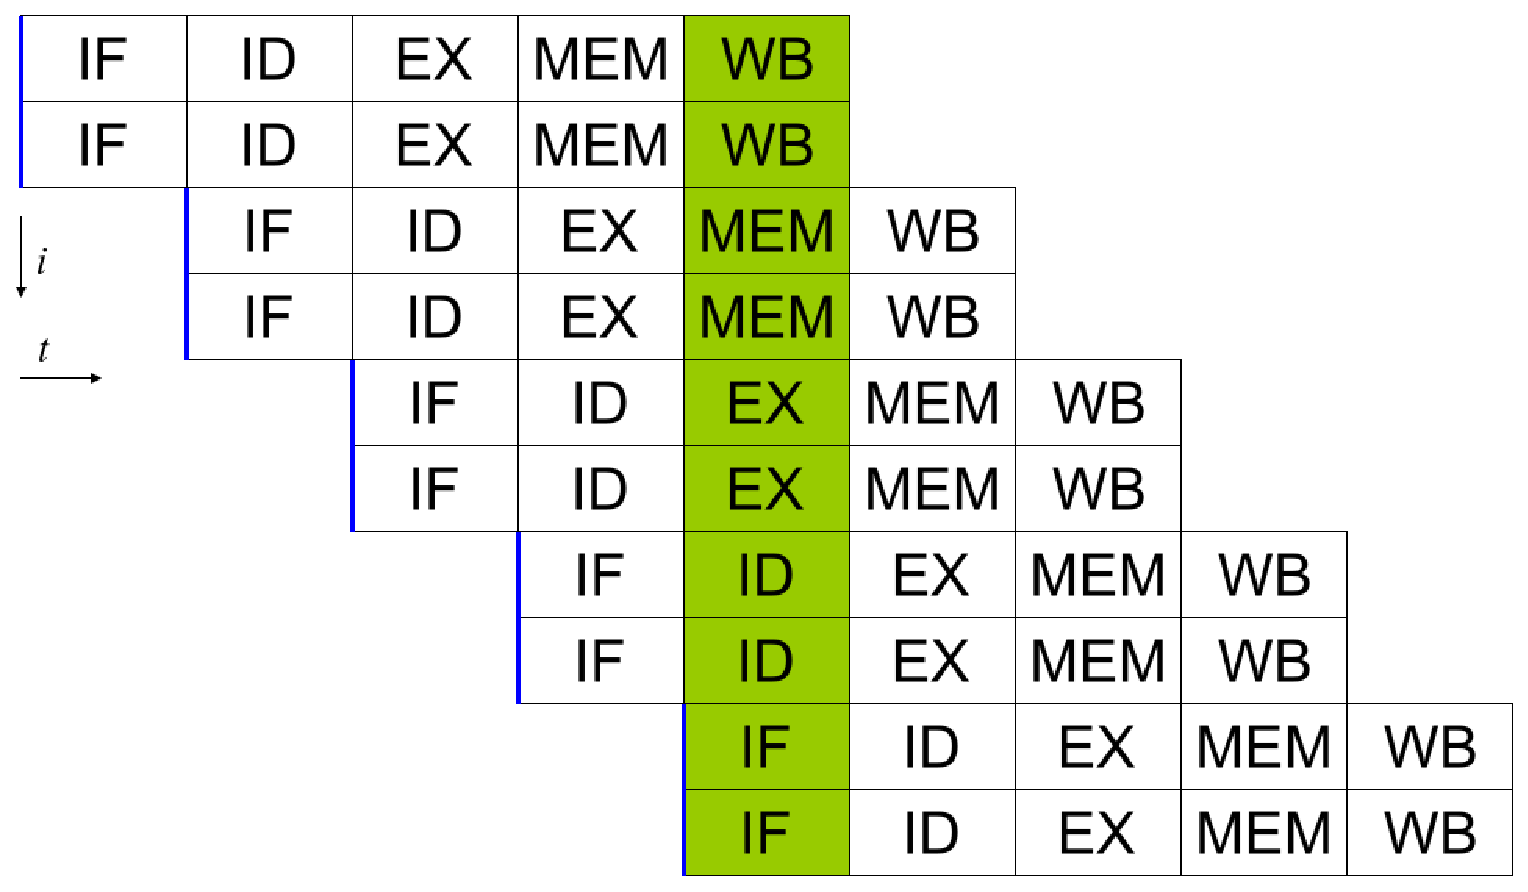
\includegraphics[width=0.55\textwidth]{img/11.superscalar_pipeline.pdf}
        \caption{Иллюстрация для Classic RISC pipeline, хотя типичный современный RISC для этого простоват}
    \end{figure}

    \pause

    В 1993 г. — Pentium I, Intel x86

    \begin{outline}{itemize}
        \1 Два АЛУ
        \1 Два конвейера, которые их «кормят»
        \1 Компилятор старается располагать рядом независимые инструкции
    \end{outline}

    \defn{Суперскалярность}{возможность автоматического распараллеливания независимых близлежащих команд в машинном коде}
\end{frame}

\begin{frame}[fragile]{Суперскалярное исполнение: пример}
    Пример: запись на стек параметров функции при помощи команд \mintinline{as}{mov}, а не \mintinline{as}{push}, поскольку соседние \mintinline{as}{push} изменяют состояние стека $\Rightarrow$ зависимы

    C:
    \begin{minted}{c}
        f(0, 1, 5, 8);
    \end{minted}

    Ассемблер x86 (32 бита):
    \begin{minted}{as}
        ; Без оптимизации vs с оптимизацией
                             sub esp, 16
        push 8               mov DWORD PTR [ebp -08h], 8
        push 5               mov DWORD PTR [ebp -0Bh], 5
        push 1               mov DWORD PTR [ebp -10h], 1
        push 0               mov DWORD PTR [ebp -14h], 0
        call f               call f
    \end{minted}

    Суперскалярный процессор может параллельно исполнить \mintinline{as}{mov} из примера
\end{frame}

\subsection{Very Long Instructoin Word}

\begin{frame}{VLIW}
    \defn{Very Long Instruction Word}{подход к проектированию архитектур, подразумевающий явное распараллеливание независимых близлежащих команд в машинном языке}

    \begin{itemize}
        \item Yale Multiflow, 1980-е
        \item Эльбрус 3, 1993
        \item Intel Itanium, 2001
        \item Современные DSP и GPU
    \end{itemize}

    Похоже на \emph{микропрограммирование}: в одной машинной команде несколько инструкций для разных блоков процессора, которые задействуются параллельно. Не все блоки разные: м.б. несколько АЛУ, несколько математических сопроцессоров и т.д.
\end{frame}

\subsection{Внеочередное исполнение}

\begin{frame}{Внеочередное исполнение}
    \defn{Внеочередное исполнение (Out of Order execution)}{способ выполнения машинных команд не в порядке следования, а в порядке
    готовности к исполнению}

    Впервые: Cray CDC 6600, 1963 г. При приблизительно тех же разрядности и
    тактовой частоте CDC 6600 был существенно быстрее БЭСМ-6, у которой был
    конвейер. Но и гораздо сложнее и дороже.

    Идея: поток инструкций программы делится на:

    \begin{enumerate}
        \tightlist
        \item
        Последовательность инструкций, к выполнению которых ещё не приступали
        \item
        Инструкции, которыми «занимаются»
        \item
        «Отработанные» инструкции
    \end{enumerate}

    \pause

    Почти как конвейер, но интеллектуальнее: «текущий» фрагмент программы
    пропускается не через конвейер, а через «окно», в котором происходит
    гораздо больше всего.
\end{frame}

\begin{frame}{Современный пример: Intel Core i7}
        \begin{enumerate}
            \tightlist
            \item
            Очередная команда разбивается на микрооперации
            \item
            Если фактически независимые микрооперации работают с одними и теми же
            регистрами, для них выделяются разные экземпляры регистров (стадия
            \emph{переименования регистров})
            \item
            Микрооперации помещаются в Reorder Buffer и переупорядочиваются, в
            т.ч. с микрооперациями близлежащих команд
            \item
            Микрооперации поступают на 6 исполнительных блоков
        \end{enumerate}

        Это делает процессорное ядро Intel OOO
\end{frame}

\begin{frame}{Современный пример: Архитектура Intel OOO}
    \begin{figure}
        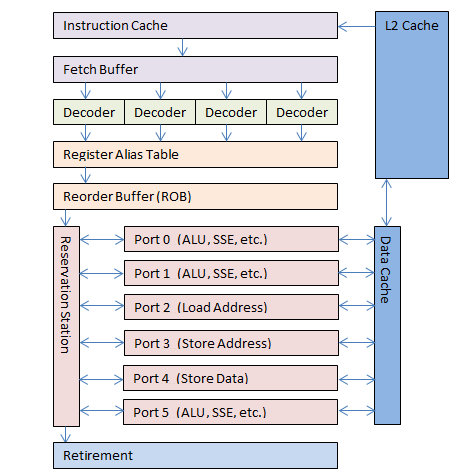
\includegraphics[height=0.8\textheight]{img/11.Intel_OOO.png}
    \end{figure}
\end{frame}

\begin{frame}{Дальнейшее развитие Intel OOO}
        Впервые OOO применили в Pentium Pro в 1995 г.

        \begin{itemize}
            \tightlist
            \item
            У Intel x86 достаточно сложный машинный код, из-за этого простаивали
            исполнительные блоки, а блок выборки за ними не успевал
        \end{itemize}

        \pause

        Идея: можно сделать два блока выборки и исполнять два потока на одном
        наборе исполнительных блоков

        Запатентована в Sun Microsystems в 1994 г., впервые в серийных
        микропроцессорах реализована в Intel в 2002 г., технология названа \emph{Intel
        Hyperthreading}

        Одно ядро для программиста и ОС выглядит, как два
\end{frame}

\begin{frame}{Intel HyperThreading}
    \begin{figure}
        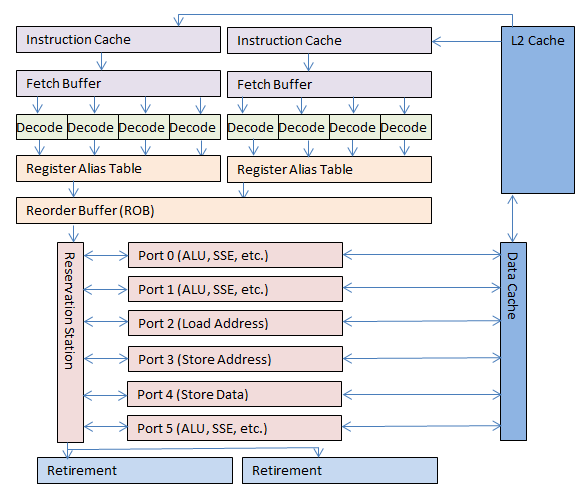
\includegraphics[height=0.8\textheight]{img/11.Intel_HT.png}
    \end{figure}

    \href{https://habr.com/ru/post/182002/}{Путешествие через вычислительный конвейер процессора} (перевод)
\end{frame}

\begin{frame}{Внеочередное исполнение в современных RISC}
    Многие современные RISC процессоры, например, последние ARM и \emph{отдельные реализации} RISC-V, не только     обнаруживают конфликты, но и переупорядочивают инструкции, и выполняют
    прочие аналогичные оптимизации.

    Причина?..

    \pause

    В условиях параллельного выполнения программ на компилятор положиться
    уже не получится, т.к. полная информация о последовательности операций
    доступна лишь во время выполнения.

    MIPS, даже современные, часто одноядерные, поэтому могут не обрабатывать конфликты конвейера (помните \mintinline{as}{nop}?)
\end{frame}

\section{Немного мимими: стековые архитектуры}

\begin{frame}{Идея стековой архитектуры}
    Идея: постфиксная запись операций. Операции либо добавляют данные на стек, либо преобразуют несколько элементов с вершины стека, и помещают на вершину результат
\end{frame}

\begin{frame}{Примеры стековых архитектур}
    \begin{outline}[itemize]
        \1 Языки программирования и виртуальные машины
            \2 Forth, PostScript и некоторые современные
            \2 Lilith (Вирт, Паскаль), AVE (ЛГУ, Алгол68), Java, .NET CLR, CPython и некоторые другие В.М.
        \1 Калькуляторы
            \2 Калькуляторы HP (с 1970-х – н.в.)
            \2 Калькуляторы МК-61, МК-52 (1980-е – 90-е) и МК-161, МК-152 (2000-е – н.в.)
        \1 Компьютеры
            \2 Самсон (Терехов, ЛГУ), Кронос (Котов, Новосибирск) — 1980-е
            \2 ЛИСП-машины — 1980-е
            \2 Процессор Intel Itanium (он также VLIW) — 2000-e
            \2 Бестактовый процессор GA144 для Forth
    \end{outline}
\end{frame}

\begin{frame}{Преимущества и недостатки стековых архитектур}
    \begin{itemize}
        \item Преимущества: красиво, легко писать компиляторы
        \item Недостаток: проблемы с распараллеливанием, неудобный произвольный доступ к верхрим элементам стека (не случайно Itanium VLIW!)
    \end{itemize}
\end{frame}

\section*{}

\begin{frame}{Вопросы и упражнения}
\begin{block}{Вопросы}
\begin{itemize}
\tightlist
\item Назовите и определите основные блоки процессора.
\item Что такое вычислительный конвейер?
\item Во сколько раз может максимально ускорить выполнение программы конвейер, выполняющий команды в 3 этапа?
\item Назовите виды конфликтов конвейера.
\item Как RISC-процессоры разрешают конфликты конвейера?
\item Как CISC-процессоры разрешают конфликты конвейера?
\item Дайте определение суперскалярной архитектуре.
\item Что такое VLIW?
\item Что такое внеочередное исполнение машинных команд?
\item В чём идея технологии HyperThreading?
\item Почему современные многоядерные RISC сами разрешают конфликты конвейера?
\item Что такое стековая архитектура, каковы преимущества и недостатки стековых архитектур?
\item Приведите примеры стековых архитектур.
\end{itemize}
\end{block}
\end{frame}

\postamble

\end{document}
